\documentclass{article}
\usepackage[margin=0.9in]{geometry}
\usepackage{amsmath}
\usepackage{amssymb}
\usepackage{booktabs}
\usepackage{xintexpr}
\usepackage{tikz}
\usetikzlibrary{arrows,automata}
\usepackage{subcaption}
\usepackage{float}
\usepackage{fancyhdr}

\pagestyle{fancy}
\lhead{Tanner Hobson}
\rhead{thobson2}

\newcommand{\T}{1}
\newcommand{\F}{0}
\newcommand{\TF}[1]{\if1#1\T\else\F\fi}
\newcommand{\xintTF}[1]{\xintifboolexpr{#1}{\T}{\F}}

\newcommand{\logicrule}[2]{
\begin{array}{l}
#1 \\
\midrule
\therefore #2 \\
\end{array}
}

\newcommand{\inv}[1]{#1^{-1}}

\renewcommand{\d}[1]{\,\textnormal{d}#1}
\newcommand{\dd}[2]{\frac{\d{#1}}{\d{#2}}}
\newcommand{\ddd}[2]{\dfrac{\d{#1}}{\d{#2}}}

\DeclareMathOperator{\var}{Var}
\DeclareMathOperator{\E}{\mathcal{E}}

\newcommand{\multistep}[1]{\begin{array}{rl} #1 \end{array}}
\newcommand{\subeq}{\subseteq}
\newcommand{\sub}{\subset}

\newcommand{\conj}[1]{\overline{#1}}

\newcommand{\problem}[1]{$\boxed{\textbf{#1}}$}

\setlength\parindent{0pt}
\setlength\parskip{0em}

\begin{document}

\begin{minipage}{\textwidth}
\problem{2.1a}

\begin{figure}[H]
  \centering
  \begin{subfigure}{.5\textwidth}
    \centering
    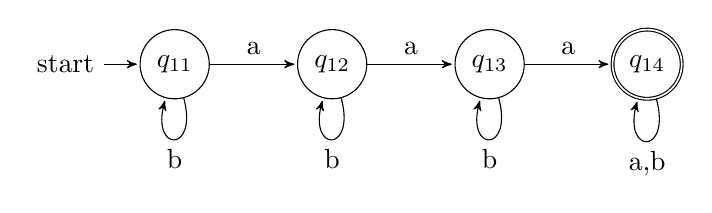
\begin{tikzpicture}[>=stealth',shorten >=1pt,auto,node distance=2cm]
      \node[initial,state] (q11) {$q_{11}$};
      \node[state] (q12) [right of=q11] {$q_{12}$};
      \node[state] (q13) [right of=q12] {$q_{13}$};
      \node[state,accepting] (q14) [right of=q13] {$q_{14}$};

      \path[->]
      (q11) edge node {a} (q12)
      (q11) edge [loop below] node {b} (q11)

      (q12) edge node {a} (q13)
      (q12) edge [loop below] node {b} (q12)

      (q13) edge node {a} (q14)
      (q13) edge [loop below] node {b} (q13)

      (q14) edge [loop below] node {a,b} (q14)
      ;
    \end{tikzpicture}
    \caption{$M_{1a}$}
  \end{subfigure}%
  %
  \begin{subfigure}{.5\textwidth}
    \centering
    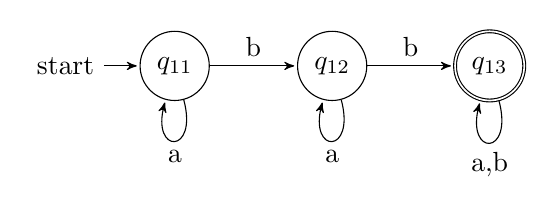
\begin{tikzpicture}[>=stealth',shorten >=1pt,auto,node distance=2cm]
      \node[initial,state] (q11) {$q_{11}$};
      \node[state] (q12) [right of=q11] {$q_{12}$};
      \node[state,accepting] (q13) [right of=q12] {$q_{13}$};

      \path[->]
      (q11) edge [loop below] node {a} (q11)
      (q11) edge node {b} (q12)

      (q12) edge [loop below] node {a} (q12)
      (q12) edge node {b} (q13)

      (q13) edge [loop below] node {a,b} (q13)
      ;
    \end{tikzpicture}
    \caption{$M_{1b}$}
  \end{subfigure}

  \begin{subfigure}{1\textwidth}
    \centering
    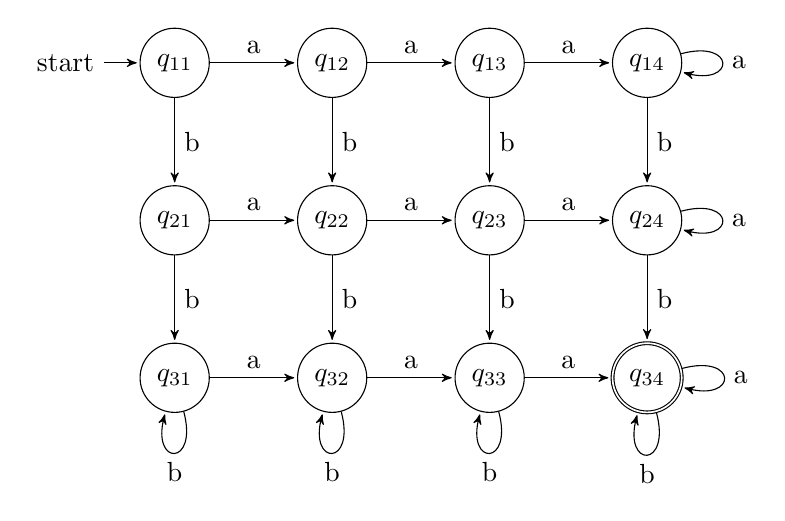
\begin{tikzpicture}[>=stealth',shorten >=1pt,auto,node distance=2cm]
      \node[initial,state] (q11) {$q_{11}$};
      \node[state] (q12) [right of=q11] {$q_{12}$};
      \node[state] (q13) [right of=q12] {$q_{13}$};
      \node[state] (q14) [right of=q13] {$q_{14}$};

      \node[state] (q21) [below of=q11] {$q_{21}$};
      \node[state] (q22) [below of=q12] {$q_{22}$};
      \node[state] (q23) [below of=q13] {$q_{23}$};
      \node[state] (q24) [below of=q14] {$q_{24}$};

      \node[state] (q31) [below of=q21] {$q_{31}$};
      \node[state] (q32) [below of=q22] {$q_{32}$};
      \node[state] (q33) [below of=q23] {$q_{33}$};
      \node[state,accepting] (q34) [below of=q24] {$q_{34}$};

      \path[->]
      (q11) edge node {a} (q12)
      (q11) edge node {b} (q21)

      (q12) edge node {a} (q13)
      (q12) edge node {b} (q22)

      (q13) edge node {a} (q14)
      (q13) edge node {b} (q23)

      (q14) edge [loop right] node {a} (q14)
      (q14) edge node {b} (q24)
      ;

      \path[->]
      (q21) edge node {a} (q22)
      (q21) edge node {b} (q31)

      (q22) edge node {a} (q23)
      (q22) edge node {b} (q32)

      (q23) edge node {a} (q24)
      (q23) edge node {b} (q33)

      (q24) edge [loop right] node {a} (q24)
      (q24) edge node {b} (q34)
      ;

      \path[->]
      (q31) edge node {a} (q32)
      (q31) edge [loop below] node {b} (q31)

      (q32) edge node {a} (q33)
      (q32) edge [loop below] node {b} (q32)

      (q33) edge node {a} (q34)
      (q33) edge [loop below] node {b} (q33)

      (q34) edge [loop right] node {a} (q34)
      (q34) edge [loop below] node {b} (q34)
      ;
    \end{tikzpicture}
    \caption{$M_1$}
  \end{subfigure}
\end{figure}
\end{minipage}

\begin{minipage}{\textwidth}
\problem{2.1b}

\begin{figure}[H]
  \centering
  \begin{subfigure}{.5\textwidth}
    \centering
    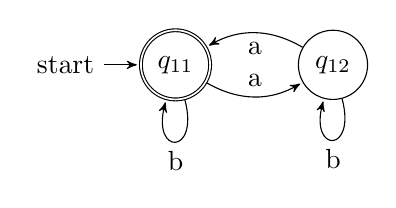
\begin{tikzpicture}[>=stealth',shorten >=1pt,auto,node distance=2cm]
      \node[initial,state,accepting] (q11) {$q_{11}$};
      \node[state] (q12) [right of=q11] {$q_{12}$};

      \path[->]
      (q11) edge [bend right] node {a} (q12)
      (q11) edge [loop below] node {b} (q11)

      (q12) edge [bend right] node {a} (q11)
      (q12) edge [loop below] node {b} (q12)
      ;
    \end{tikzpicture}
    \caption{$M_{2a}$}
  \end{subfigure}%
  %
  \begin{subfigure}{.5\textwidth}
    \centering
    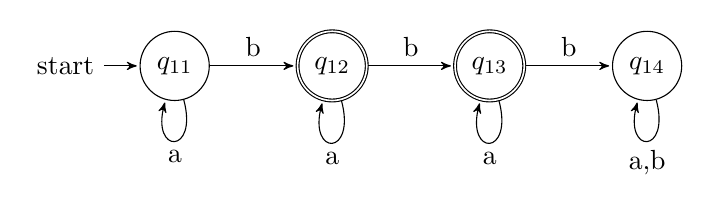
\begin{tikzpicture}[>=stealth',shorten >=1pt,auto,node distance=2cm]
      \node[initial,state] (q11) {$q_{11}$};
      \node[state,accepting] (q12) [right of=q11] {$q_{12}$};
      \node[state,accepting] (q13) [right of=q12] {$q_{13}$};
      \node[state] (q14) [right of=q13] {$q_{14}$};

      \path[->]
      (q11) edge [loop below] node {a} (q11)
      (q11) edge node {b} (q12)

      (q12) edge [loop below] node {a} (q12)
      (q12) edge node {b} (q13)

      (q13) edge [loop below] node {a} (q13)
      (q13) edge node {b} (q14)

      (q14) edge [loop below] node {a,b} (q14)
      ;
    \end{tikzpicture}
    \caption{$M_{2b}$}
  \end{subfigure}

  \begin{subfigure}{1\textwidth}
    \centering
    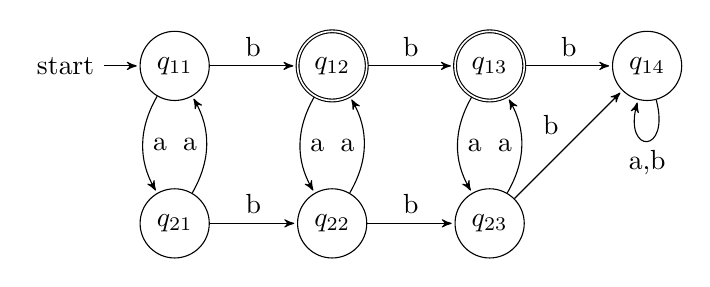
\begin{tikzpicture}[>=stealth',shorten >=1pt,auto,node distance=2cm]
      \node[initial,state] (q11) {$q_{11}$};
      \node[state,accepting] (q12) [right of=q11] {$q_{12}$};
      \node[state,accepting] (q13) [right of=q12] {$q_{13}$};
      \node[state] (q14) [right of=q13] {$q_{14}$};

      \node[state] (q21) [below of=q11] {$q_{21}$};
      \node[state] (q22) [below of=q12] {$q_{22}$};
      \node[state] (q23) [below of=q13] {$q_{23}$};

      \path[->]
      (q11) edge node {b} (q12)
      (q11) edge [bend right] node {a} (q21)

      (q12) edge node {b} (q13)
      (q12) edge [bend right] node {a} (q22)

      (q13) edge node {b} (q14)
      (q13) edge [bend right] node {a} (q23)

      (q21) edge node {b} (q22)
      (q21) edge [bend right] node {a} (q11)

      (q22) edge node {b} (q23)
      (q22) edge [bend right] node {a} (q12)

      (q23) edge node {b} (q14)
      (q23) edge [bend right] node {a} (q13)

      (q14) edge [loop below] node {a,b} (q14)
      ;
    \end{tikzpicture}
    \caption{$M_2$}
  \end{subfigure}
\end{figure}
\end{minipage}

\begin{minipage}{\textwidth}
\problem{2.1c}

\begin{figure}[H]
  \centering
  \begin{subfigure}{.5\textwidth}
    \centering
    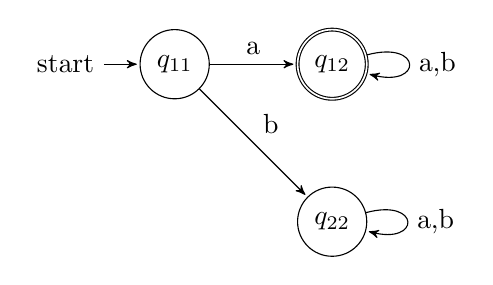
\begin{tikzpicture}[>=stealth',shorten >=1pt,auto,node distance=2cm]
      \node[initial,state] (q11) {$q_{11}$};
      \node[state,accepting] (q12) [right of=q11] {$q_{12}$};

      \node[state] (q22) [below of=q12] {$q_{22}$};

      \path[->]
      (q11) edge node {a} (q12)
      (q11) edge node {b} (q22)

      (q12) edge [loop right] node {a,b} (q12)

      (q22) edge [loop right] node {a,b} (q22)
      ;
    \end{tikzpicture}
    \caption{$M_{3a}$}
  \end{subfigure}%
  %
  \begin{subfigure}{.5\textwidth}
    \centering
    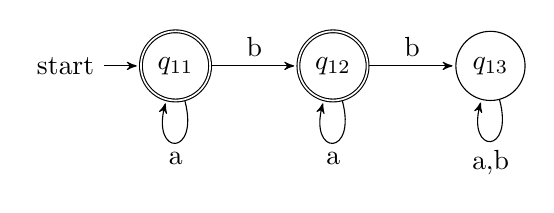
\begin{tikzpicture}[>=stealth',shorten >=1pt,auto,node distance=2cm]
      \node[initial,state,accepting] (q11) {$q_{11}$};
      \node[state,accepting] (q12) [right of=q11] {$q_{12}$};
      \node[state] (q13) [right of=q12] {$q_{13}$};

      \path[->]
      (q11) edge [loop below] node {a} (q11)
      (q11) edge node {b} (q12)

      (q12) edge [loop below] node {a} (q12)
      (q12) edge node {b} (q13)

      (q13) edge [loop below] node {a,b} (q13)
      ;
    \end{tikzpicture}
    \caption{$M_{3b}$}
  \end{subfigure}

  \begin{subfigure}{1\textwidth}
    \centering
    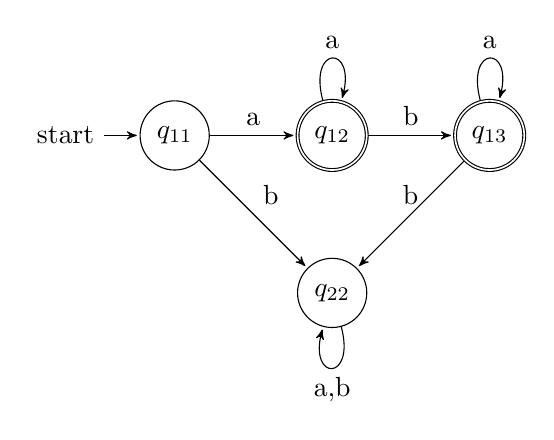
\begin{tikzpicture}[>=stealth',shorten >=1pt,auto,node distance=2cm]
      \node[initial,state] (q11) {$q_{11}$};
      \node[state,accepting] (q12) [right of=q11] {$q_{12}$};
      \node[state,accepting] (q13) [right of=q12] {$q_{13}$};

      \node[state] (q22) [below of=q12] {$q_{22}$};

      \path[->]
      (q11) edge node {a} (q12)
      (q11) edge node {b} (q22)

      (q12) edge [loop above] node {a} (q12)
      (q12) edge node {b} (q13)

      (q13) edge [loop above] node {a} (q13)
      (q13) edge node [above] {b} (q22)

      (q22) edge [loop below] node {a,b} (q22)
      ;
    \end{tikzpicture}
    \caption{$M_3$}
  \end{subfigure}
\end{figure}
\end{minipage}

\begin{minipage}{\textwidth}
\problem{2.2a}

\begin{figure}[H]
  \centering
  \begin{subfigure}{.5\textwidth}
    \centering
    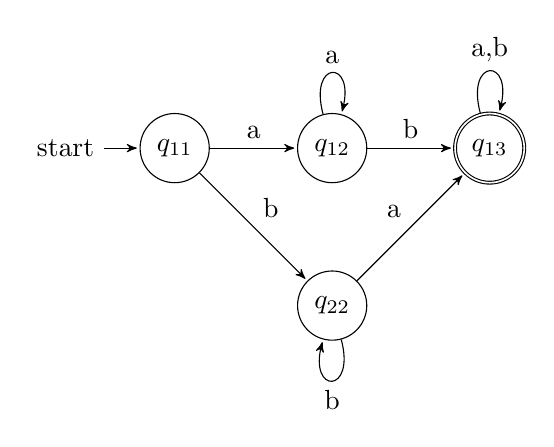
\begin{tikzpicture}[>=stealth',shorten >=1pt,auto,node distance=2cm]
      \node[initial,state] (q11) {$q_{11}$};
      \node[state] (q12) [right of=q11] {$q_{12}$};
      \node[state,accepting] (q13) [right of=q12] {$q_{13}$};

      \node[state] (q22) [below of=q12] {$q_{22}$};

      \path[->]
      (q11) edge node {a} (q12)
      (q11) edge node {b} (q22)

      (q12) edge [loop above] node {a} (q12)
      (q12) edge node {b} (q13)

      (q13) edge [loop above] node {a,b} (q13)

      (q22) edge [loop below] node {b} (q22)
      (q22) edge node {a} (q13)
      ;
    \end{tikzpicture}
    \caption{$M_1$}
  \end{subfigure}%
  %
  \begin{subfigure}{.5\textwidth}
    \centering
    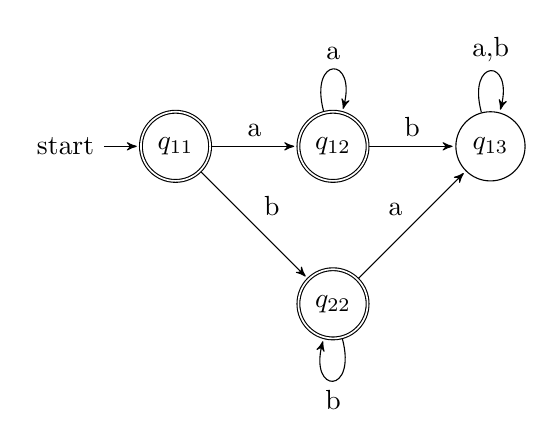
\begin{tikzpicture}[>=stealth',shorten >=1pt,auto,node distance=2cm]
      \node[initial,state,accepting] (q11) {$q_{11}$};
      \node[state,accepting] (q12) [right of=q11] {$q_{12}$};
      \node[state] (q13) [right of=q12] {$q_{13}$};

      \node[state,accepting] (q22) [below of=q12] {$q_{22}$};

      \path[->]
      (q11) edge node {a} (q12)
      (q11) edge node {b} (q22)

      (q12) edge [loop above] node {a} (q12)
      (q12) edge node {b} (q13)

      (q13) edge [loop above] node {a,b} (q13)

      (q22) edge [loop below] node {b} (q22)
      (q22) edge node {a} (q13)
      ;
    \end{tikzpicture}
    \caption{$\neg{}M_1$}
  \end{subfigure}
\end{figure}
\end{minipage}

\begin{minipage}{\textwidth}
\problem{2.2b}

\begin{figure}[H]
  \centering
  \begin{subfigure}{.5\textwidth}
    \centering
    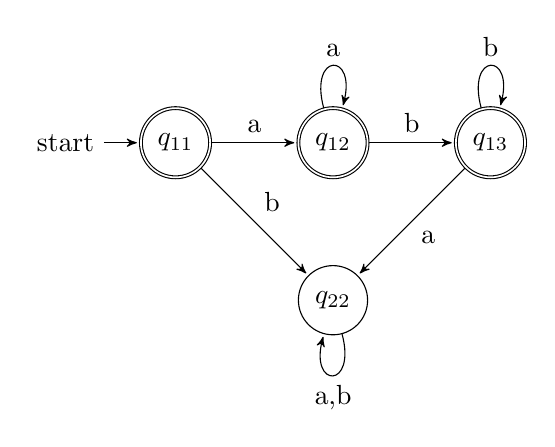
\begin{tikzpicture}[>=stealth',shorten >=1pt,auto,node distance=2cm]
      \node[initial,state,accepting] (q11) {$q_{11}$};
      \node[state,accepting] (q12) [right of=q11] {$q_{12}$};
      \node[state,accepting] (q13) [right of=q12] {$q_{13}$};

      \node[state] (q22) [below of=q12] {$q_{22}$};

      \path[->]
      (q11) edge node {a} (q12)
      (q11) edge node {b} (q22)

      (q12) edge [loop above] node {a} (q12)
      (q12) edge node {b} (q13)

      (q13) edge [loop above] node {b} (q13)
      (q13) edge node {a} (q22)

      (q22) edge [loop below] node {a,b} (q22)
      ;
    \end{tikzpicture}
    \caption{$M_2$}
  \end{subfigure}%
  %
  \begin{subfigure}{.5\textwidth}
    \centering
    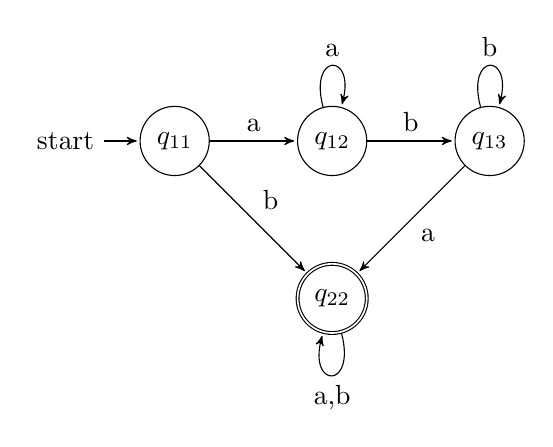
\begin{tikzpicture}[>=stealth',shorten >=1pt,auto,node distance=2cm]
      \node[initial,state] (q11) {$q_{11}$};
      \node[state] (q12) [right of=q11] {$q_{12}$};
      \node[state] (q13) [right of=q12] {$q_{13}$};

      \node[state,accepting] (q22) [below of=q12] {$q_{22}$};

      \path[->]
      (q11) edge node {a} (q12)
      (q11) edge node {b} (q22)

      (q12) edge [loop above] node {a} (q12)
      (q12) edge node {b} (q13)

      (q13) edge [loop above] node {b} (q13)
      (q13) edge node {a} (q22)

      (q22) edge [loop below] node {a,b} (q22)
      ;
    \end{tikzpicture}
    \caption{$\neg{}M_2$}
  \end{subfigure}
\end{figure}
\end{minipage}

\begin{minipage}{\textwidth}
\problem{2.2c}

\begin{figure}[H]
  \centering
  \begin{subfigure}{.5\textwidth}
    \centering
    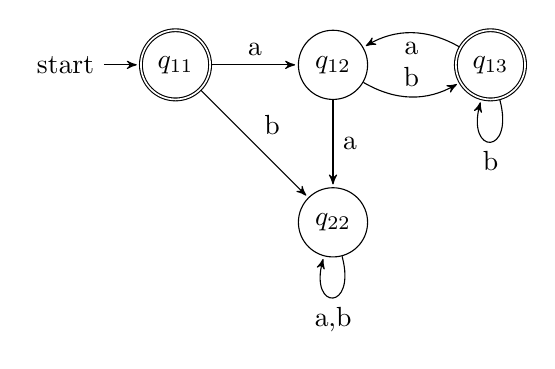
\begin{tikzpicture}[>=stealth',shorten >=1pt,auto,node distance=2cm]
      \node[initial,state,accepting] (q11) {$q_{11}$};
      \node[state] (q12) [right of=q11] {$q_{12}$};
      \node[state,accepting] (q13) [right of=q12] {$q_{13}$};

      \node[state] (q22) [below of=q12] {$q_{22}$};

      \path[->]
      (q11) edge node {a} (q12)
      (q11) edge node {b} (q22)

      (q12) edge node {a} (q22)
      (q12) edge [bend right] node {b} (q13)

      (q13) edge [loop below] node {b} (q13)
      (q13) edge [bend right] node {a} (q12)

      (q22) edge [loop below] node {a,b} (q22)
      ;
    \end{tikzpicture}
    \caption{$M_3$}
  \end{subfigure}%
  %
  \begin{subfigure}{.5\textwidth}
    \centering
    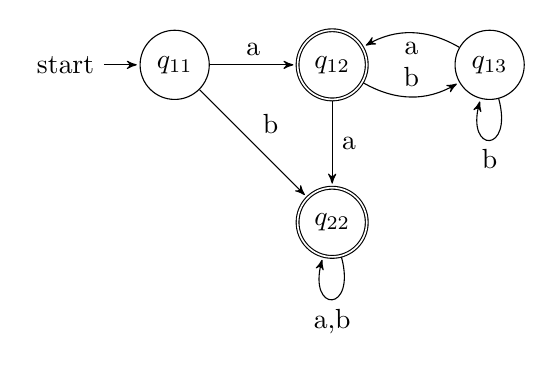
\begin{tikzpicture}[>=stealth',shorten >=1pt,auto,node distance=2cm]
      \node[initial,state] (q11) {$q_{11}$};
      \node[state,accepting] (q12) [right of=q11] {$q_{12}$};
      \node[state] (q13) [right of=q12] {$q_{13}$};

      \node[state,accepting] (q22) [below of=q12] {$q_{22}$};

      \path[->]
      (q11) edge node {a} (q12)
      (q11) edge node {b} (q22)

      (q12) edge node {a} (q22)
      (q12) edge [bend right] node {b} (q13)

      (q13) edge [loop below] node {b} (q13)
      (q13) edge [bend right] node {a} (q12)

      (q22) edge [loop below] node {a,b} (q22)
      ;
    \end{tikzpicture}
    \caption{$\neg{}M_3$}
  \end{subfigure}
\end{figure}
\end{minipage}

\end{document}
